\chapter{Introduction}\label{ch:introduction}
% Achieving intelligence requires modeling the real world,
% this is true in the context of scientific research but also of engineering tools.
Ever since the beginning of our existence, we have always been curious to understand the complexity of the world we live in.
This is not only true at the individual level as we keep building and improving our knowledge over our lifespan,
but also at the level of humankind where common intelligence has never really stopped rising since the beginning of civilization.
Science, an objectification of our curiousity, aims at grounding the construction of this common knowledge to rationality. In particular, the modern scientific method
arguably relies on 5 pillars as depicted in \Cref{fig:ch01:scientific_method} which ensure discoveries are made out of rigor and on the basis of current scientific knowledge.
Although the scientific method can answer questions in the context of a specified model of the world as stated by the hypotheses, the more fundamental goal of science is to refine these models by critisizing their ability to predict the real world. In this context, the aim of this thesis is to explore and contribute to modern techniques for building or refining these models of the world.
% This thesis is about this: How can we automatically combine scientific knowledge and data to create faithful and useful models?
\begin{figure}[h]
  \centering
  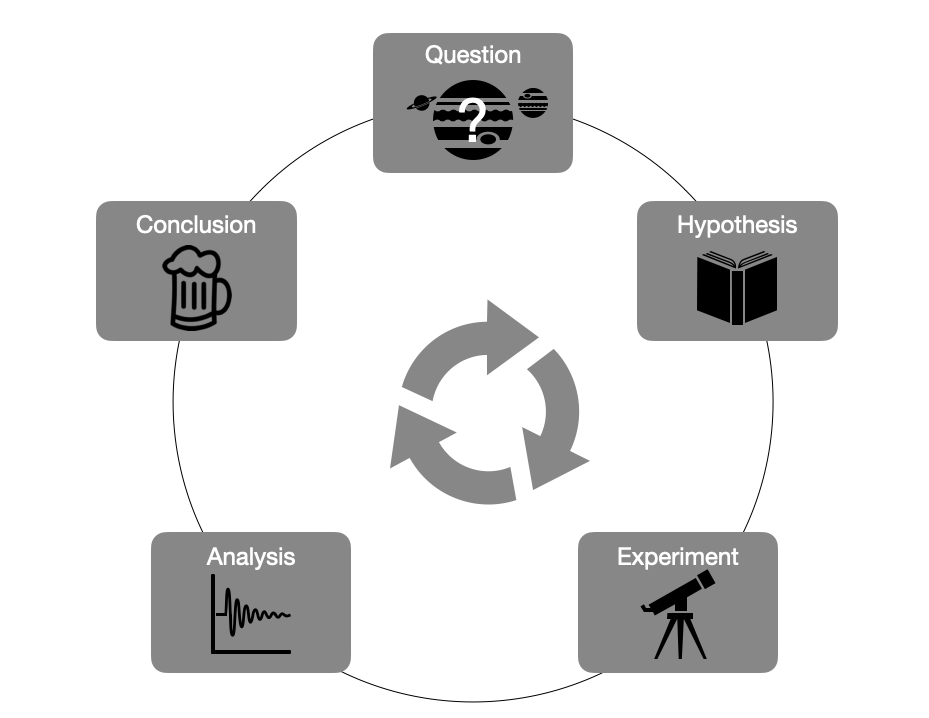
\includegraphics[width=.8\textwidth]{figures/chapter01/trapist_disco.png}
  \caption{Illustration of the scientific inquiry as a simplified 5-steps process.
  The pictograms sketch a cartoon of the TRAPPIST-1 planetary system discovery made by astronomers from Li{\`e}ge university in 2016 \citep{gillon2017seven}.
  A scientist first formulates a \textit{research question} and a set of reasonable \textit{hypotheses}, together they define a class of hypothetical models of the world.
  In order to answer his question, he gathers data from \textit{experiments} and analyze them in the context of his modeling assumptions. Checking the consistency of diffent hypothetical models allows him \textit{to provide an answer} to his initial question up to a certain degree of certainty.}
  \label{fig:ch01:scientific_method}
\end{figure}

Classically, grounded on their domain expertise, scientists or engineers would incrementally complexify existing models to improve their faithfulness to reality. The scientific method then applied would validate or reject the new class of models.
This strategy has not only led to today's state of science but also to the uttermost engineering accomplishments of modern times.
In engineering, these successes range from impacting our daily life such as by enpowering it with nuclear electricity - as predicted by special relativity - to
allowing ones to read this manuscript on a smart tablet - thanks to Maxwell equations' implications on the design of modern computers.
More abstract but arguably as impactful on our vision of the universe, the classical model refinment strategy led to all modern scientific breakthroughs at the moment of writing this manuscript. These models allow astronomers to observe the furthest human-known objects, thanks to general relativity and gravitational lensing, and enable the indirect observations of black holes thanks to gravitational waves theory.

% A word somewhere that scientific models are usually probabilistic generative models because good models require modeling uncertainty coming from unmodeled phenomenon or phenomenon
% that are only modeled up to a certain level of stochasticity. Introduced the concept of explicit generative vs implicit generative models


Despite these numerous achievements, the classical modelling approach has recently been challenged by machine learning. Where humans fall short to find patterns in large amount of data and to build arbitrarily complex models, machines enpowered by modern machine learning perform these tasks naturally days and nights.
On the one hand, this paradigm shift from hand-crafted to automated modeling happens in a world where the most ambitious scientific experiments generate petabytes ($10^{15}$) of data per seconds \citep{noauthor_cern_nodate} and the computing capacity keeps increasing exponentially. At the same time, the human brain has not changed since Galileo Galilei, the father of modern science, and is unfortunately not wired to aprehend such vast amount of data. On the other hand, deep learning has now proven its ability to build accurate generative models that outperform the ones designed out of human expertise. This is for example true in the context of voice synthesis \citep{van_den_oord_wavenet_2016}, text-translation \citep{GPT3, bert...}, chat bots, or even text-to-image synthesis \citep{Dall-e-2, imagen}, to cite a few. Under these cirumstances, the paradigm shift, even in a scientific context, seems natural.

% Paragraph arguing that we still need to work on deep generative models as they are not perfect yet.
Although machine learning has recently shined in the aforementioned applications, there still exist many obstacles to the regular application of machine learning modeling as a replacement to hand-crafted models. One limitation concerns the expressivity of deep generative models and the inherent difficulty that comes with optimizing these large models.
As a matter of facts explicit models often lack expressivity. This is the price to pay for requiring a direct access to the model's likelihood.
In opposition to explicit models, implicit models are very expressive and arguably model almost any complex generative process. However optimizing such models is usually very hard and achieving a high quality synthesis requires an good understanding of potential numerical issues and tricks to avoid them. Most of these problems arise indirectly from the fact that these models do not provide access to their likelihood.
In the first part of this thesis, we study this concern, demonstrating the limitation of existing approaches and providing solutions to improve the expressivity of some class of
models.

% Paragraph Arguing generative models are not data efficient because they do not built on common knowledge as would do a human
Even granted with perfect optimization procedures and universal generative models, the problem would not be solved. To fight the curse of dimensionality
we need strong inductive bias. But more than the curse of dimensionality we also often requires these models to not stupidly fall as soon as they are required to
act in an environment slightly different from the training configuration. We want these models to be able to built on current knowledge. It may also be important that these Models
have a level of interpretability for humans especially if we want to use them in a scientific context. The second part of this thesis study this equally important aspect.


% Historically modeling was achieved by manually describing sub-part of the studied processed with simple physical equations.
% Machine learning led to a paradigm shift in this context.

% The aim of this thesis is to study and improve generative modeling in this context (paradigm shift from hand crafted to automated modeling).
% Two aspects of improments are proposed
% 1) Improving and studying the expressivity of automated probabilistic modeling approaches.
% 2) Combining domain knowledge with data driven approaches to achieve faithful and generalizable modeling.
% Both aspects are as important as on the one hand the availability of data increases for many problems which opens the path to breakthrough in the modeling of complex phenomenon.
% On the second hand, data are usually biased in some sense and generalization outside of this can only happen by enforcing invariance or equivariance with respect to spme aspects of the problems or real world.
\section{Research questions}


\section{Outline and contributions}

\section{Publications}
Setting aside this introduction, an original primer on probabilistic modeling in \chapref{02} and the conclusion,
the scientific content of this manuscript is exclusively borrowed to original contributions I made to generative modeling over the last 4 years.
Each selected contribution sets its own chapter complemented with a prologue and an epilogue.
The manuscript builds upon the following list of publications:

\begin{itemize}
\item[] \citep{wehenkel_unconstrained_2019} \textit{Unconstrained monotonic neural networks},
\textbf{Wehenkel Antoine} and Louppe Gilles.\\
Advances in neural information processing systems, 2019.\\
$\quad \rightarrow$ \chapref{05}.

\item[] \citep{wehenkel_you_2020} \textit{You say Normalizing Flows I see Bayesian Networks},
\textbf{Wehenkel Antoine} and Louppe Gilles.\\
International Conference on Machine Learning, Workshop on Invertible Neural Networks, Normalizing Flows, and Explicit Likelihood Models, 2020.\\
$\quad \rightarrow$ \chapref{04}.

\item[] \citep{wehenkel2021graphical} \textit{Graphical Normalizing Flows},
\textbf{Wehenkel Antoine} and Louppe Gilles.\\
International Conference on Artificial Intelligence and Statistics, 2021.\\
$\quad \rightarrow$ \chapref{06}.

\item[] \citep{wehenkel2021diffusion} \textit{Diffusion Priors In Variational Autoencoders},
\textbf{Wehenkel Antoine} and Louppe Gilles.\\
International Conference on Machine Learning, Workshop on Invertible Neural Networks, Normalizing Flows, and Explicit Likelihood Models, 2021.\\
$\quad \rightarrow$ \chapref{03}.

\item[] \citep{wehenkel2022robust} \textit{Robust Hybrid Learning With Expert Augmentation},
\textbf{Wehenkel Antoine}, Behrmann Jens, Hsu Hsiang, Sapiro Guillermo, Louppe Gilles, and Jacobsen J{\"o}rn-Henrik.\\
In preparation, arXiv preprint arXiv:2202.03881.\\
$\quad \rightarrow$ \chapref{07}.

\end{itemize}

Along the pursuit of my PhD degree, I had the chance to take part in fruitful collaborations not directly related to the scope of this thesis.
The following list of co-authored publications stemmed from these collaborations:
\begin{itemize}
\item[] \citep{pesah2018recurrent} \textit{Recurrent Machines For Likelihood-free Inference},
Arthur Pesah, \textbf{Wehenkel Antoine} and Louppe Gilles.\\
Advances in neural information processing systems, MetaLearn Workshop, 2018.

\item[] \citep{wehenkel2020parameter} \textit{Parameter Estimation Of Three-phase Untransposed Short Transmission Lines From Synchrophasor Measurements},
\textbf{Wehenkel Antoine}, Mukhopadhyay Arpan, Le Boudec Jean-Yves, Paolone Mario.\\
IEEE Transactions on Instrumentation and Measurement, 2020.

\item[] \citep{vecoven2020introducing} \textit{Introducing Neuromodulation In Deep Neural Networks To Learn Adaptive Behaviours},
Vecoven Nicolas, Ernst Damien, \textbf{Wehenkel Antoine}, Drion Guillaume.\\
PloS one 15 (1), e0227922.

\item[] \citep{vandegar2021neural} \textit{Neural Empirical Bayes: Source Distribution Estimation and its Applications to Simulation-Based Inference},
Vandegar Maxime, Kagan Michael, \textbf{Wehenkel Antoine} and Louppe Gilles.\\
International Conference on Artificial Intelligence and Statistics, 2021.

\item[] \citep{delaunoy2020lightning} \textit{Lightning-Fast Gravitational Wave Parameter Inference through Neural Amortization},
Delaunoy Arnaud, \textbf{Wehenkel Antoine}, Hinderer Tanja, Nissanke Samaya, Weniger Christoph, Williamson Andrew R and Louppe Gilles.\\
Advances in neural information processing systems, ML4Science Workshop, 2020.

\item[] \citep{hermans2021averting} \textit{Averting A Crisis In Simulation-based Inference},
Hermans Joeri, Delaunoy Arnaud, Rozet Fran{\c{c}}ois, \textbf{Wehenkel Antoine} and Louppe Gilles.\\
In preparation, arXiv preprint arXiv:2110.06581.

\item[] \citep{dumas2021probabilistic} \textit{A Probabilistic Forecast-driven Strategy For A Risk-aware Participation In The Capacity Firming Market},
Dumas Jonathan, Cointe Colin, \textbf{Wehenkel Antoine}, Sutera Antonio, Fettweis Xavier and Corn{\'e}lusse Bertrand.\\
IEEE Transactions on Sustainable Energy, 2021.

\item[] \citep{dumas2022deep} \textit{A Deep Generative Model For Probabilistic Energy Forecasting In Power Systems: Normalizing Flows},
Dumas Jonathan, \textbf{Wehenkel Antoine}, Lanaspeze Damien, Corn{\'e}lusse Bertrand and Sutera Antonio.\\
Applied Energy, 2022.

\end{itemize}
